%% abtex2-modelo-artigo.tex, v-1.9.6 laurocesar
%% Copyright 2012-2016 by abnTeX2 group at http://www.abntex.net.br/ 
%%
%% This work may be distributed and/or modified under the
%% conditions of the LaTeX Project Public License, either version 1.3
%% of this license or (at your option) any later version.
%% The latest version of this license is in
%%   http://www.latex-project.org/lppl.txt
%% and version 1.3 or later is part of all distributions of LaTeX
%% version 2005/12/01 or later.
%%
%% This work has the LPPL maintenance status `maintained'.
%% 
%% The Current Maintainer of this work is the abnTeX2 team, led
%% by Lauro César Araujo. Further information are available on 
%% http://www.abntex.net.br/
%%
%% This work consists of the files abntex2-modelo-artigo.tex and
%% abntex2-modelo-references.bib
%%

% ------------------------------------------------------------------------
% ------------------------------------------------------------------------
% abnTeX2: Modelo de Artigo Acadêmico em conformidade com
% ABNT NBR 6022:2003: Informação e documentação - Artigo em publicação 
% periódica científica impressa - Apresentação
% ------------------------------------------------------------------------
% ------------------------------------------------------------------------

\documentclass[
	article,			% indica que é um artigo acadêmico
	12pt,				% tamanho da fonte
	oneside,			% para impressão apenas no recto. Oposto a twoside
	a4paper,			% tamanho do papel. 
	% -- opções da classe abntex2 --
	%chapter=TITLE,		% títulos de capítulos convertidos em letras maiúsculas
	%section=TITLE,		% títulos de seções convertidos em letras maiúsculas
	%subsection=TITLE,	% títulos de subseções convertidos em letras maiúsculas
	%subsubsection=TITLE % títulos de subsubseções convertidos em letras maiúsculas
	% -- opções do pacote babel --
	english,			
	brazil,
	sumario=tradicional
	]{abntex2}


% ---
% PACOTES
% ---

% ---
% Pacotes fundamentais 
% ---
\usepackage{lmodern}			% Usa a fonte Latin Modern
\usepackage[T1]{fontenc}		% Selecao de codigos de fonte.
\usepackage[utf8]{inputenc}		% Codificacao do documento (conversão automática dos acentos)
\usepackage{indentfirst}		% Indenta o primeiro parágrafo de cada seção.
\usepackage{nomencl} 			% Lista de simbolos
\usepackage{color}				% Controle das cores
\usepackage{graphicx}			% Inclusão de gráficos
\usepackage{microtype} 			% para melhorias de justificação

% ---
		
% ---
% Pacotes adicionais, usados apenas no âmbito do Modelo Canônico do abnteX2
% ---
\usepackage{lipsum}				% para geração de dummy text
% ---
		
% ---
% Pacotes de citações
% ---
\usepackage[brazilian,hyperpageref]{backref}	 % Paginas com as citações na bibl
\usepackage[alf]{abntex2cite}	% Citações padrão ABNT
% ---

% ---
% Configurações do pacote backref
% Usado sem a opção hyperpageref de backref
\renewcommand{\backrefpagesname}{Citado na(s) página(s):~}
% Texto padrão antes do número das páginas
\renewcommand{\backref}{}
% Define os textos da citação
\renewcommand*{\backrefalt}[4]{
	\ifcase #1 %
		Nenhuma citação no texto.%
	\or
		Citado na página #2.%
	\else
		Citado #1 vezes nas páginas #2.%
	\fi}%
% ---

% ---
% Informações de dados para CAPA e FOLHA DE ROSTO
% ---
\titulo{Suíte de testes\\para biblioteca de engenharia}
\autor{Jonhnatha Trigueiro}
\local{Brasil}
\data{2016}
% ---

% ---
% Configurações de aparência do PDF final

% alterando o aspecto da cor azul
\definecolor{blue}{RGB}{41,5,195}

% informações do PDF
\makeatletter
\hypersetup{
     	%pagebackref=true,
		pdftitle={\@title}, 
		pdfauthor={\@author},
    	pdfsubject={Modelo de artigo científico com abnTeX2},
	    pdfcreator={LaTeX with abnTeX2},
		pdfkeywords={abnt}{latex}{abntex}{abntex2}{atigo científico}, 
		colorlinks=true,       		% false: boxed links; true: colored links
    	linkcolor=blue,          	% color of internal links
    	citecolor=blue,        		% color of links to bibliography
    	filecolor=magenta,      		% color of file links
		urlcolor=blue,
		bookmarksdepth=4
}
\makeatother
% --- 

% ---
% compila o indice
% ---
\makeindex
% ---

% ---
% Altera as margens padrões
% ---
\setlrmarginsandblock{3cm}{3cm}{*}
\setulmarginsandblock{3cm}{3cm}{*}
\checkandfixthelayout
% ---

% --- 
% Espaçamentos entre linhas e parágrafos 
% --- 

% O tamanho do parágrafo é dado por:
\setlength{\parindent}{1.3cm}

% Controle do espaçamento entre um parágrafo e outro:
\setlength{\parskip}{0.2cm}  % tente também \onelineskip

% Espaçamento simples
\SingleSpacing

% ----
% Início do documento
% ----
\begin{document}

% Seleciona o idioma do documento (conforme pacotes do babel)
%\selectlanguage{english}
\selectlanguage{brazil}

% Retira espaço extra obsoleto entre as frases.
\frenchspacing 

% ----------------------------------------------------------
% ELEMENTOS PRÉ-TEXTUAIS
% ----------------------------------------------------------

%---
%
% Se desejar escrever o artigo em duas colunas, descomente a linha abaixo
% e a linha com o texto ``FIM DE ARTIGO EM DUAS COLUNAS''.
% \twocolumn[    		% INICIO DE ARTIGO EM DUAS COLUNAS
%
%---
% página de titulo
\maketitle

% resumo em português
\begin{resumoumacoluna}
É proposto a criação uma suite de testes para Biblioteca de Engenharia. Atualmente a biblioteca é de difícil manutenção, consequentemente de lento desenvolvimento. Esta abordará a reforma da biblioteca e os passos necessários para torná-la testável, servindo de base para desenvolvimento colaborativo. Será iniciado um novo projeto com CMake, versionado no GIT e Publicado no GitHUB. Será configurado o Integrador contínuo TravisCI para a realização do processo de \textit{build}, executando os testes em nuvem. Tem-se como objetivo a redução do tempo de desenvolvimento, aumento da confiabilidade de código e desacoplamento do código, padrão em projetos opensource.

 \vspace{\onelineskip}
 
 \noindent
 \textbf{Palavras-chave}: Teste, Desenvolvimento Orientado à Testes, Integração Contínua
\end{resumoumacoluna}

% resumo em inglês
\begin{resumo}[Abstract]
 \begin{otherlanguage*}{english}
   It's proposed creating a test suite to a Engineering Library. Actually this library is difficult to maintain, accordingly of slow development. This will approach the reforming of library and the steps needed to make it testable, serving as base to collaborative development. Will be started a new CMake, GIT versioned project published at GitHUB. Also will be configured TravisCI Continuous Integration service for building process, executing on cloud tests. Has as goal reduce development time, raising code confiability and code decoupling, standard in opensource projects.

   \vspace{\onelineskip}
 
   \noindent 
   \textbf{Key-words}: Testing, Test Driven Development, Continuous Integration.
 \end{otherlanguage*}
\end{resumo}

\textual

% ----------------------------------------------------------
% Introdução
% ----------------------------------------------------------
\section*{Introdução}
\addcontentsline{toc}{section}{Introdução}

Desenvolvimento guiado à testes é um processo de criação de software
que se baseia na repetição de um ciclo de desenvolvimento muito curto e definido.
Como objetivos dessa abordagem se pode citar os seguintes: Produtividade no desenvolvimento,
código fonte de fácil manutenção e confiabilidade do código.

A integração contínua, na prática, é uma técnica de mesclar o código de vários desenvolvedores em uma linha comum compartilhada de forma a ser feito várias vezes ao dia. Foi proposto inicialmente por Grady Booch em seu método 1991 e é usado com muita intensidade no método de desenvolvimento ágil XP, que advoga realizar o processo de integração continua mais de uma vez por dia.

A biblioteca de Engenharia foi criada na intenção de tornar prático os conhecimentos adquiridos durante o curso de Engenharia de computação. Esta possui um conjunto de implementações que precisam ser mantidas por uma série de futuros profissionais.

A abordagem de concepção de softwares guiado à testes será implementada sobre a Biblioteca, dispondo-se das melhores ferramentas para se atingir tal objetivo. Isto incluirá os seguintes pontos:

\begin{itemize}
	\item{Organização do repositório GIT atual}
	\item{Inclusão das classes de teste na biblioteca}
	\item{Configuração da ferramenta de integração contínua para realização dos testes}
	\item{Gerar documentação para novos desenvolvedores utilizarem e contribuírem com a ferramenta}
\end{itemize}

O foco deste projeto visa a criação de uma metodologia de trabalho assim como a utilização de uma série de ferramentas visando a consolidação do método proposto.

Como resultado, o presente projeto visa alcançar os seguintes objetivos:
\begin{itemize}
	\item{Tornar a biblioteca segura, ou seja, garantir que seu funcionamento seja conforme esperado;}
	\item{Aumentar a participação de desenvolvedores na construção e utilização da biblioteca e}
	\item{Reduzir o custo de implementação, uma vez que este tende a aumentar exponencialmente com o acréscimo da complexidade.}
\end{itemize}

\pagebreak
\section{Definições}

Será utilizado um conjunto de ferramentas e serviços para o objetivo proposto, citados à seguir:

\subsection{C++}

Linguagem de programação, compilada, multi-paradigma de uso geral, criada em 1979 por Bjarne Stroustrup, padronizada em 1998. Será a linguagem de programação escolhida para o desenvolvimento do estudo.

O site oficial linguagem é \href{http://www.cplusplus.com/}{http://www.cplusplus.com/}

\pagebreak
\subsection{Biblioteca de Engenharia}

Biblioteca inicialmente criada pelo professor Doutor André Dantas com foco em ferramentas matemáticas para ajudar a compreensão do curso de Engenharia de Computação. Escrita em C++ conta com classes fundamentais para o processamento dos dados, como manipulação de Matrizes e Polinômios. Esta será a ferramenta de trabalho na qual criaremos a suíte de testes.

Também é previsto para a biblioteca, como planejamento para os futuros recursos:

\begin{itemize}
	\item Representar modelos matemáticos para sistemas conhecidos;
	\item Sintonizar sistemas dado modelo escolhido, método de sintonia e entrada de dados, achando melhor combinação;
\end{itemize}

O link para biblioteca: \href{https://github.com/EngineeringLibrary/ECO}{https://github.com/EngineeringLibrary/ECO}

\pagebreak
\subsection{CMAKE}
É um sistema de gestão de \textit{build} de projetos. É livre de plataforma e opensource. Foi designado para suportar hierarquias de diretório e aplicativos que dependam de outras bibliotecas. É usado em conjunto com meios de \textit{build}, como o make, Xcode da Apple e o Visual Studio da Microsoft. Tem dependências mínimas. Requer apenas um compilador C++ no seu próprio sistema de \textit{build}.

O CMake pode localizar executáveis, arquivos e bibliotecas. Essas localizações são armazenadas em um cache que pode ser refinado antes de gerar os arquivos de \textit{build}.

O CMAKE é utilizado em grandes projetos opensource: Blender, CLion, cURL, LLVM e Clang, OpenCV e ZeroMQ são exemplos de projetos.

\pagebreak
\subsection{SSH}
É um protocolo de rede encriptado operando na camada 7 do modelo OSI. Permite o login remoto e possibilidade de se operar outros serviços por meio desta através de redes não seguras.

Esta provê um canal seguro em uma arquitetura cliente-servidor. Aplicações do SSH incluem:

\begin{itemize}
	\item{Login em linha de comando;}
	\item{Execução remota de comandos;}
	\item{Transferência segura de arquivos e}
	\item{Tunelamento de serviços através de rede criptografada.}
\end{itemize}

O SSH foi projetado para ser uma substituição para o Telnel e para protocolos de shell remotos inseguros, como os protocolos Berkeley rlogin, rsh e rexec.

\pagebreak
\subsection{GIT}

Ferramenta de controle de versão criado por \textbf{Linus Torvalds} em 2005. É amplamente utilizada para desenvolvimento de software e outras tarefas de controle de versão. É um sistema distribuído de controle de revisão com ênfase na velocidade e não concomitante ao repositório remoto. 

O design desse projeto foi a síntese da experiência de Torvalds com o projeto Linux. Ele precisava manter um projeto largo e distribuído ao mesmo tempo que precisava de um ambiente de trabalho funcional. Pra isso adotou as seguintes características de implementação:

\subsubsection{Suporte Forte para desenvolvimento não linear}
Possui suporte rápido para ramificação (branching) e mesclagem (merging) e inclui ferramentas específicas para visualizar e navegar no histórico de desenvolvimento de modo a poder reconstruir toda a arvore de commits. Commit é um conjunto de alterações feita em um código fonte.

\begin{figure}[!h]
\centering
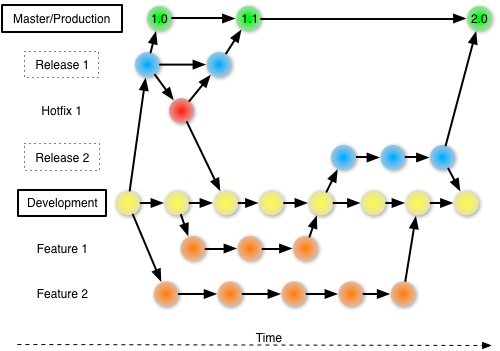
\includegraphics[scale=0.5]{images/git_workflow.png}
\caption{Exemplo de desenvolvimento não linear. Linhas horizontais seriam as branches. Bolinhas, commits, setas entre as branchs, operações de Merge}
\label{img_git_workflow}
\end{figure}

\subsubsection{Ambiente Distribuído}

O GIT dá à cada desenvolvedor uma cópia local de todo o histórico de desenvolvimento. Essas modificações são importadas como branches adicionais de desenvolvimento e podem ser mescladas da mesma forma feita localmente.

\subsubsection{Compatibilidade com os protocolos de rede existentes}
Repositório é o nome dado ao local de trabalho do GIT. Repositórios podem ser publicados via protocolo HTTP, FTP, rsync (até a versão 2.8.0), a um protocolo GIT utilizando socket ou SSH. Este último é amplamente utilizado por sua segurança e flexibilidade.

\subsubsection{Manipulação eficiente de grandes projetos}
Linus Torvalds descreve que o GIT como sendo rápido e escalável. A coleta de histórico de alterações pode ser extremamente rápida pelo simples fato de ser realizada localmente, dado sua natureza Distribuída.

\subsubsection{Autenticação Criptografada do histórico}
O histórico do GIT é armazenado de forma que uma versão particular (um commit) depende do seu histórico completo até o presente commit. Este ganha uma assinatura garantindo que versões anteriores não sejam substituídas sem que se seja notado.

\subsubsection{Design baseado em \textit{Toolkit} e estratégias plugáveis de mesclagem de código}
O GIT foi projetado com um conjunto de programas escritos em C e uma série de \textit{shell scripts} que produzem \textit{wrappers} nestes aplicativos. Sua concepção desacoplada torna fácil a atuação em cadeia de várias aplicações para se atingir o objetivo desejado.

O git possui uma forma bem definida de modelo de mesclagem de código. Existem muitos algorítmos que se conectam ao modelo que finalizam o processo de mesclagem. Caso nenhuma das estratégias existentes funcionem a própria ferramenta se encarrega de iniciar o modo manual de mesclagem de código, onde o desenvolvedor "resolve" o conflito.

\subsubsection{Resíduos se armazenam a não ser que sejam limpos}
O foco do GIT é fazer com que os dados não sejam perdidos. Abortar operações ou reverter à versões anteriores do código podem deixar trechos de código sem utilização pelo repositório. Por padrão o GIT mantém esses códigos, por menores que sejam, na sua estrutura a não ser rotinas de limpeza sejam executadas.

\subsubsection{Compactação periódica de código}
Git armazena cada novo arquivo criado como um arquivo separado. Compactar arquivos individualmente torna o processo lento e ineficiente. Como estratégia para otimização de tempo, o GIT empacota grupos de arquivos em unidades chamadas \textit{packfile} e as compacta aumentando drásticamente a velocidade do repositório.






\pagebreak
\subsection{GitHub}
É um serviço de hospedagem de projetos que utilizam o GIT como sistema de controle de versionamento. Este é um dos serviços mais utilizados no mundo por desenvolvedores, sendo posicionado como 65$^{\circ}$ lugar no hanking do Alexa.

Apesar de fundamentalmente o Github ser utilizado para hospedagem de código, este possui os seguintes recursos:

\begin{itemize}
	\item{Documentação, incluindo renderização de código Markdown em uma variedade grande de formatos}
\end{itemize}

\pagebreak
\subsection{Teste}

O conceito de teste é abrangente. Vias gerais, significa firmar convicção de um juiz sobre a verdade dos fatos alegados pelas partes em juízo. Em programação este termo pode ser lido como "a convicção do desenvolvedor" sobre a confiabilidade de que o sistema desenvolvido irá funcionar conforme esperado.

Há algumas fases para o teste de software. Cada um visa abranger um escopo no ciclo de desenvolvimento. Podemos citar os seguintes:
\begin{itemize}
	\item Teste de unidade;
	\item Teste de integração;
	\item Teste de sistema;
	\item Teste de aceitação e
	\item Teste de operação.
\end{itemize}

A rotina de testes, apesar de ser de fácil compreensão, requer disciplina por parte do desenvolvedor, que, precisa pensar em código fracamente acoplado. Leia-se "código fracamente acoplado" aquele o qual os as funcionalidades são dispostas em funções, com entradas e saídas simpels, de modo que se comprometa a realizar apenas uma competência.

\subsubsection{Teste de unidade}

É o menor grupo de testes. Estes testam funções específicas. Dado uma entrada e saída conhecidas pelo desenvolvedor, a suite de testes comparará o resultado da aplicação da função com a saída esperada. Dependendo do método de asserção escolhido, o teste irá passar ou falhar.

\pagebreak
\subsection{CXXTest}
É um framework de testes unitários para C++ que é similar, em essência, ao JUnit, CppUnit e xUnit. É de fácil utilização porque não requer precompilar a biblioteca de teste. Também não requer recursos avançados, como RTTI por exemplo, e possui uma forma bastante flexível de descoberta de testes.

\pagebreak
\subsection{TravisCI}
É um serviço se integração contínua usado para executar o processo de build e teste de projetos de software geralmente hospedados no GitHub.

% ----------------------------------------------------------
% Seção de explicações
% ----------------------------------------------------------

\pagebreak
\section{Desenvolvimento}

\subsection{Problemática}

A atual biblioteca possui vários colaboradores. Várias classes da mesma possuem dependências de bibliotecas de base. Um exemplo é a classe de Operações Matriciais que depende da classe de Matriz, por exemplo. Garantir que esta classe esteja funcionanco é crucial para a criação de novas Classes, que dependem destas.

Se faz necessário garantir a evolução da biblioteca, com muitos colaboradores de modo que a mesma possa ter a garantia de ser utilizada funcionando conforme esperado.

Conforme o código fonte vai se tornando maior, o nível de complexidade do algorítmo cresce e a possibilidade de se implantar erros aumenta. Um código não coberto por testes implica que este passará a se tornar de difícil compreensão, consequentemente levando à novas implementações cada vez mais lentas e onerosas para o time.


\subsection{Metodologia}
Com base no problema proposto se faz necessário utilizar a abordagem do desenvolvimento orientado à testes (TDD, do inglês "Test Driven Development"), que consiste em uma aplicação que fará o teste do software em questão com base em suas classes e métodos em um algorítmo de teste unitário.

Como o já existe um código legado, o mesmo precisa ser preparado para que este possa se tornar testável. Este comportamento é incomum relacionado à definição de desenvolvimento guiado à testes:

\begin{citacao}
The test-driven development strategy 
requires writing automated tests prior to 
developing functional code in small, rapid 
iterations.
	\cite[Introduction]{testdrivendevelopment.1}
\end{citacao}

O projeto será formatado utilizando o \textit{CMake}. Este, por sua vez, organizará todo o código fonte do projeto de forma que seja agnóstico de compilador, ou seja, qualquer IDE será capaz de utilizar esse código fonte e, dependendo da arquitetura e compilador utilizado, o cmake será capaz de gerar a estrutura do projeto para o alvo. 

O teste, por sua vez, é realizado com a suíte de testes \textbf{CXXTest}, através de um processo que consiste em dois passos:

\begin{itemize}
	\item{Criação de um arquivo de header com as macros do CXXTEST realizando os testes de asserção;}
	\item{Execução do comando intermédiário da biblioteca que adicionará aos headers a lógica necessária para o funcionamento da biblioteca, e por fim,}
	\item{Compilação e execução da suíte de testes que nos retornará um sumário de erros ou sucesso da ferramenta}
\end{itemize}

Com isso, integraremos tanto o código fonte quanto o código dos testes do projeto no GIT e faremos o \textit{push} desse repositório para o \textit{GitHUB}. Neste passo, teremos integrado ao projeto um serviço de build que estará escutando o repositório através de \textit{Webhooks} e disparará uma tarefa de coletar o último commit e executará a rotina de teste proposta.


%% ADICIONAR INFO SOBRE BENEFICIOS DO PROCESSO COMO RESULTADO ESPERADO %%

%\subsection{Processo de desenvolvimento}
%\subsubsection{Planejamento para desenvolvimento do projeto}


% ---
% Finaliza a parte no bookmark do PDF, para que se inicie o bookmark na raiz
% ---
\bookmarksetup{startatroot}% 
% ---

% ---
% Conclusão
% ---
%\section*{Considerações finais}
%\addcontentsline{toc}{section}{Considerações finais}

%\lipsum[1]

%\begin{citacao}
%\lipsum[2]
%\end{citacao}

%\lipsum[3]

% ----------------------------------------------------------
% ELEMENTOS PÓS-TEXTUAIS
% ----------------------------------------------------------
\postextual

% ----------------------------------------------------------
% Referências bibliográficas
% ----------------------------------------------------------
\pagebreak
\bibliography{artigo_joey}
\nocite{cpluspluscom.1}
\nocite{cmakeorg.1}
\nocite{gitscm.1}
\nocite{gitscm.2}
\nocite{gitscm.3}
\nocite{gitscm.4}
\nocite{gitscm.5}
\nocite{gitscm.6}


% ----------------------------------------------------------
% Glossário
% ----------------------------------------------------------
%
% Há diversas soluções prontas para glossário em LaTeX. 
% Consulte o manual do abnTeX2 para obter sugestões.
%
%\glossary

% ----------------------------------------------------------
% Apêndices
% ----------------------------------------------------------

% ---
% Inicia os apêndices
% ---
%\begin{apendicesenv}

% ----------------------------------------------------------
%\chapter{Nullam elementum urna vel imperdiet sodales elit ipsum pharetra ligula
%ac pretium ante justo a nulla curabitur tristique arcu eu metus}
% ----------------------------------------------------------
%\lipsum[55-57]

%\end{apendicesenv}
% ---

% ----------------------------------------------------------
% Anexos
% ----------------------------------------------------------
\cftinserthook{toc}{AAA}

% ---
% Inicia os anexos
% ---
%\anexos

%\begin{anexosenv}
%
%% ---
%\chapter{Cras non urna sed feugiat cum sociis natoque penatibus et magnis dis
%parturient montes nascetur ridiculus mus}
%% ---
%
%\lipsum[31]
%
%\end{anexosenv}

\end{document}